


\tikzset{every picture/.style={line width=0.75pt}} %set default line width to 0.75pt        

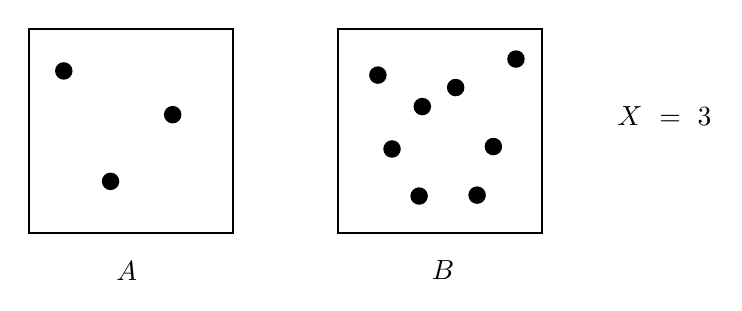
\begin{tikzpicture}[x=0.75pt,y=0.75pt,yscale=-1,xscale=1]
%uncomment if require: \path (0,928); %set diagram left start at 0, and has height of 928

%Shape: Square [id:dp9704491284322827] 
\draw  [color={rgb, 255:red, 0; green, 0; blue, 0 }  ,draw opacity=1 ] (185.93,89.16) -- (284.28,89.16) -- (284.28,187.5) -- (185.93,187.5) -- cycle ;
%Shape: Square [id:dp03136999448950761] 
\draw   (334.93,89.16) -- (433.28,89.16) -- (433.28,187.5) -- (334.93,187.5) -- cycle ;
%Shape: Circle [id:dp7080864036358405] 
\draw  [fill={rgb, 255:red, 0; green, 0; blue, 0 }  ,fill opacity=1 ] (199.13,109.5) .. controls (199.13,107.46) and (200.79,105.8) .. (202.83,105.8) .. controls (204.88,105.8) and (206.53,107.46) .. (206.53,109.5) .. controls (206.53,111.55) and (204.88,113.21) .. (202.83,113.21) .. controls (200.79,113.21) and (199.13,111.55) .. (199.13,109.5) -- cycle ;
%Shape: Circle [id:dp47838494517380514] 
\draw  [fill={rgb, 255:red, 0; green, 0; blue, 0 }  ,fill opacity=1 ] (350.46,111.5) .. controls (350.46,109.46) and (352.12,107.8) .. (354.16,107.8) .. controls (356.21,107.8) and (357.87,109.46) .. (357.87,111.5) .. controls (357.87,113.55) and (356.21,115.21) .. (354.16,115.21) .. controls (352.12,115.21) and (350.46,113.55) .. (350.46,111.5) -- cycle ;
%Shape: Circle [id:dp7883825334163144] 
\draw  [fill={rgb, 255:red, 0; green, 0; blue, 0 }  ,fill opacity=1 ] (416.99,103.77) .. controls (416.99,101.72) and (418.65,100.07) .. (420.7,100.07) .. controls (422.74,100.07) and (424.4,101.72) .. (424.4,103.77) .. controls (424.4,105.81) and (422.74,107.47) .. (420.7,107.47) .. controls (418.65,107.47) and (416.99,105.81) .. (416.99,103.77) -- cycle ;
%Shape: Circle [id:dp9074461888124206] 
\draw  [fill={rgb, 255:red, 0; green, 0; blue, 0 }  ,fill opacity=1 ] (221.66,162.7) .. controls (221.66,160.66) and (223.32,159) .. (225.36,159) .. controls (227.41,159) and (229.07,160.66) .. (229.07,162.7) .. controls (229.07,164.75) and (227.41,166.41) .. (225.36,166.41) .. controls (223.32,166.41) and (221.66,164.75) .. (221.66,162.7) -- cycle ;
%Shape: Circle [id:dp6890015089873274] 
\draw  [fill={rgb, 255:red, 0; green, 0; blue, 0 }  ,fill opacity=1 ] (370.33,169.77) .. controls (370.33,167.72) and (371.99,166.07) .. (374.03,166.07) .. controls (376.08,166.07) and (377.73,167.72) .. (377.73,169.77) .. controls (377.73,171.81) and (376.08,173.47) .. (374.03,173.47) .. controls (371.99,173.47) and (370.33,171.81) .. (370.33,169.77) -- cycle ;
%Shape: Circle [id:dp8947912143724381] 
\draw  [fill={rgb, 255:red, 0; green, 0; blue, 0 }  ,fill opacity=1 ] (387.93,117.5) .. controls (387.93,115.46) and (389.59,113.8) .. (391.63,113.8) .. controls (393.68,113.8) and (395.33,115.46) .. (395.33,117.5) .. controls (395.33,119.55) and (393.68,121.21) .. (391.63,121.21) .. controls (389.59,121.21) and (387.93,119.55) .. (387.93,117.5) -- cycle ;
%Shape: Circle [id:dp3696607406333412] 
\draw  [color={rgb, 255:red, 0; green, 0; blue, 0 }  ,draw opacity=1 ][fill={rgb, 255:red, 0; green, 0; blue, 0 }  ,fill opacity=1 ] (357.26,147.1) .. controls (357.26,145.06) and (358.92,143.4) .. (360.96,143.4) .. controls (363.01,143.4) and (364.67,145.06) .. (364.67,147.1) .. controls (364.67,149.15) and (363.01,150.81) .. (360.96,150.81) .. controls (358.92,150.81) and (357.26,149.15) .. (357.26,147.1) -- cycle ;
%Shape: Circle [id:dp9854982234444247] 
\draw  [fill={rgb, 255:red, 0; green, 0; blue, 0 }  ,fill opacity=1 ] (406.09,145.94) .. controls (406.09,143.89) and (407.75,142.23) .. (409.8,142.23) .. controls (411.84,142.23) and (413.5,143.89) .. (413.5,145.94) .. controls (413.5,147.98) and (411.84,149.64) .. (409.8,149.64) .. controls (407.75,149.64) and (406.09,147.98) .. (406.09,145.94) -- cycle ;
%Shape: Circle [id:dp652836802320137] 
\draw  [fill={rgb, 255:red, 0; green, 0; blue, 0 }  ,fill opacity=1 ] (251.59,130.57) .. controls (251.59,128.52) and (253.25,126.87) .. (255.3,126.87) .. controls (257.34,126.87) and (259,128.52) .. (259,130.57) .. controls (259,132.61) and (257.34,134.27) .. (255.3,134.27) .. controls (253.25,134.27) and (251.59,132.61) .. (251.59,130.57) -- cycle ;
%Shape: Circle [id:dp026221795879973975] 
\draw  [fill={rgb, 255:red, 0; green, 0; blue, 0 }  ,fill opacity=1 ] (371.86,126.67) .. controls (371.86,124.62) and (373.52,122.97) .. (375.56,122.97) .. controls (377.61,122.97) and (379.27,124.62) .. (379.27,126.67) .. controls (379.27,128.71) and (377.61,130.37) .. (375.56,130.37) .. controls (373.52,130.37) and (371.86,128.71) .. (371.86,126.67) -- cycle ;
%Shape: Circle [id:dp4909207654318646] 
\draw  [fill={rgb, 255:red, 0; green, 0; blue, 0 }  ,fill opacity=1 ] (398.26,169.34) .. controls (398.26,167.29) and (399.92,165.63) .. (401.96,165.63) .. controls (404.01,165.63) and (405.67,167.29) .. (405.67,169.34) .. controls (405.67,171.38) and (404.01,173.04) .. (401.96,173.04) .. controls (399.92,173.04) and (398.26,171.38) .. (398.26,169.34) -- cycle ;

% Text Node
\draw (226.67,199.87) node [anchor=north west][inner sep=0.75pt]    {$\text{A}$};
% Text Node
\draw (378.73,199.54) node [anchor=north west][inner sep=0.75pt]    {$\text{B}$};
% Text Node
\draw (468,125) node [anchor=north west][inner sep=0.75pt]    {$X\ =\ 3$};


\end{tikzpicture}